\documentclass[12pt]{article}

%\usepackage{palatino}

\usepackage[utf8]{inputenc}
\usepackage[T1]{fontenc}
\usepackage[sfdefault,scaled=.85, lining]{FiraSans}
\usepackage{newtxsf}
\usepackage[spanish]{babel}
\usepackage{amssymb}
\usepackage{amsmath}
\usepackage{wasysym}
\usepackage[x11names, rgb, html]{xcolor}
\usepackage{graphicx}
\usepackage{caption}
\usepackage{float}
\usepackage{adjustbox}
\usepackage{geometry}
\usepackage{upgreek}
\usepackage[scaled=.85, lining]{FiraMono}
\usepackage[noend]{algpseudocode}
\usepackage{algorithm}
\usepackage[italic]{mathastext}
\usepackage{hyperref}
\usepackage{listingsutf8}

\hypersetup{
  % hidelinks = true,   % Oculta todos los enlaces.
  colorlinks = true,   % Muestra todos los enlaces, sin bordes alrededor.
  linkcolor={black},     % Color de enlaces genéricos
  citecolor={blue!70!black},   % Color de enlaces de referencias
  urlcolor={blue!70!black}     % Color de enlaces de URL
}

\geometry{left=3cm,right=3cm,top=3cm,bottom=3cm,headheight=1cm,headsep=0.5cm}

\setlength{\parindent}{0pt}

%%% COLORES

\definecolor{50}{HTML}{FFEBEE}
\definecolor{100}{HTML}{FFCDD2}
\definecolor{200}{HTML}{EF9A9A}
\definecolor{300}{HTML}{E57373}
\definecolor{400}{HTML}{EF5350}
\definecolor{500}{HTML}{F44336}
\definecolor{600}{HTML}{E53935}
\definecolor{700}{HTML}{D32F2F}
\definecolor{800}{HTML}{C62828}
\definecolor{900}{HTML}{B71C1C}

%% Colores de Solarized

\definecolor{sbase03}{HTML}{002B36}
\definecolor{sbase02}{HTML}{073642}
\definecolor{sbase01}{HTML}{586E75}
\definecolor{sbase00}{HTML}{657B83}
\definecolor{sbase0}{HTML}{839496}
\definecolor{sbase1}{HTML}{93A1A1}
\definecolor{sbase2}{HTML}{EEE8D5}
\definecolor{sbase3}{HTML}{FDF6E3}
\definecolor{syellow}{HTML}{B58900}
\definecolor{sorange}{HTML}{CB4B16}
\definecolor{sred}{HTML}{DC322F}
\definecolor{smagenta}{HTML}{D33682}
\definecolor{sviolet}{HTML}{6C71C4}
\definecolor{sblue}{HTML}{268BD2}
\definecolor{scyan}{HTML}{2AA198}
\definecolor{sgreen}{HTML}{859900}

%% Colores del documento

\definecolor{text}{RGB}{78,78,78}
\definecolor{accent}{RGB}{129, 26, 24}

%%% LISTINGS

%% Tildes

\lstset{
  inputencoding=utf8/latin1
}

\lstset{
  % How/what to match
   sensitive=false,
  % Border (above and below)
  frame=leftline,
  rulecolor=\color{300},
  framerule=2pt,
  % Line number
  numbers=left,
  % Extra margin on line (align with paragraph)
  xleftmargin=\parindent,
  % Put extra space under caption
  belowcaptionskip=1\baselineskip,
  % Colors
  % backgroundcolor=\color{sbase3},
  basicstyle=\footnotesize\ttfamily\color{sbase00},
  keywordstyle=\color{700},
  commentstyle=\color{300},
  stringstyle=\color{500},
  numberstyle=\color{500},
  %identifierstyle=\color{500},
  % Break long lines into multiple lines?
  breaklines=true,
  % Show a character for spaces?
  showstringspaces=false,
  tabsize=2,
  xleftmargin=0.7em,
}

\renewcommand{\lstlistingname}{Código fuente}% Listing -> Algorithm

\title{Metaheurísticas\\ \Large Aprendizaje de Pesos en Características \\ \large Práctica 2: Búsqueda basada en poblaciones}
\author{Antonio Coín Castro \\ XXXXXXXXXXZ \\ XXXXXXXXXX@correo.ugr.es \\ Grupo 1 (M 17:30-19:30)}
\date{\today}

\begin{document}
\maketitle
\tableofcontents

\newpage

\newgeometry{top=3in, left=1.2in, right=1.2in}
\textit{Con el fin de mantener en un único documento toda la información relevante para esta práctica se han incluido en esta memoria las explicaciones y descripciones de los algoritmos que ya se comentaron en la memoria de la práctica anterior, así como el análisis de resultados que ya se realizó. Para separar esta información repetida se marcan en {\color{red}rojo} las secciones que no aportan nada nuevo a esta práctica.}
\restoregeometry

\newpage

\section{Descripción del problema}

En todo el desarrollo de las prácticas consideraremos el marco general de un problema de clasificación. Fijado $n \in \mathbb{N}$, un \textit{clasificador} es cualquier función $c: \mathbb{R}^n \to C$, donde $C$ es un conjunto (finito) de clases prefijadas. Consideramos además un \textit{conjunto de entrenamiento} $T \subseteq \mathbb{R}^n$ de elementos ya clasificados: para cada $t \in T$, denotamos $\Gamma(t) \in C$ a su clase, que es conocida.\\

El problema de clasificación consiste en, dado un \textit{conjunto de prueba} $T'\subseteq \mathbb{R}^n$ no observado previamente, encontrar un clasificador $c$ que maximice el número de clases correctamente clasificadas en $T'$, tras haber sido entrenado sobre los elementos de $T$.\\

Uno de los clasificadores más conocidos y más sencillos es el clasificador $k-$NN, que asigna a cada elemento la clase que más se repite entre sus $k$ vecinos más cercanos. En el caso concreto de esta práctica trabajaremos con el clasificador $1-$NN \textbf{con pesos}: a cada elemento le asignamos la clase de su vecino más cercano, pero ponderamos la distancia en función de un vector de pesos $w \in [0,1]^n$.\\

Para el cálculo de la distancia entre dos elementos de $\mathbb{R}^n$ utilizaremos la \textit{distancia euclídea} ponderada por el ya mencionado vector de pesos:

\[
    d_w(t, s) = \sqrt{\sum_{i=1}^n w_i (s_i - t_i)^2}, \quad t, s \in \mathbb{R}^n.
\]
\vspace{.5em}

La idea tras estos pesos es que midan la importancia de cada una de las características que representan las coordenadas de los elementos $n-$dimensionales considerados, asignando más peso en el cálculo de la distancia a aquellas que sean más importantes. El problema de \textbf{aprendizaje de pesos en características} persigue justamente `'aprender'' cuál debe ser el valor de cada peso en una instancia concreta del problema.\\

Para medir la bondad de un clasificador con pesos utilizamos las siguientes métricas:

\begin{itemize}
	\item La \textbf{precisión} (T). Estudiamos cuántos ejemplos del conjunto de prueba se clasifican correctamente, entrenando previamente el clasificador (que utiliza la distancia $d_w$) con el conjunto de entrenamiento.
	\item La \textbf{simplicidad} (R). Un clasificador será más simple si tiene en cuenta un menor número de características. Diremos que una característica $i \in \{1, \dots, n\}$ no se considera en el cálculo de la distancia si su peso asociado $w_i$ es menor que $0.2$. 
\end{itemize}

Así, el problema consiste en encontrar un vector de pesos $w \in [0,1]^n$ que maximice la precisión y la simplicidad, es decir, que maximice lo que llamaremos la \textit{función objetivo}:

\[
    F(w) = \alpha T(w) + (1 - \alpha) R(w).
\]

\newpage

\section{Descripción de la aplicación de los algoritmos}

En esta sección se describen los elementos comunes a todos los algoritmos desarrollados, así como los esquemas de representación de datos de entrada y soluciones. Todo el código se ha desarrollado en \verb|C++11|.


\subsection*{{\color{red}Esquemas de representación P1}}

En primer lugar, los datos de entrada se encuentran en la carpeta \verb|DATA|. Consisten en tres conjuntos de datos \textbf{ya normalizados} en formato \verb|csv|, donde cada fila representa un ejemplo con los valores de sus características separados por '\verb|;|' y el último elemento de la fila es su clase.\\

Para representar los datos en el programa se emplea una estructura \verb|Example| que recoge toda la información necesaria: un \verb|vector<double>| con los valores de cada una de las \verb|n| características del ejemplo concreto, así como un \verb|string| que representa su clase o categoría.

\begin{verbatim}
struct Example {
    vector<double> traits;
    string category;
    int n;
}
\end{verbatim}

Cada conjunto de datos se representa entonces por un \verb|vector<Example>|, y se emplea la función \verb|read_csv| para rellenar el vector, que va leyendo los archivos línea a línea.\\ 

Además, como será necesario hacer particiones de cada conjunto de datos para implementar la técnica de \textit{$K$-fold cross validation}, se proporciona la función \verb|make_partitions| que se encarga de repartir los elementos entre los $K$ conjuntos considerados, respetando la proporción original de clases. La forma de hacer esto es simplemente ir poniendo cada clase de forma cíclica en las particiones, primando el reparto equitativo de clases al reparto equitativo de elementos.\\

Por su parte, la solución es un \verb|vector<double>| del mismo tamaño que el número de categorías consideradas en cada caso. La componente $i-$ésima del vector representa el peso otorgado a la característica $i-$ésima de cada ejemplo del problema.

\subsection*{Esquemas de representación P2}
\label{representacion}
\addcontentsline{toc}{subsection}{\nameref{representacion}}

Para el desarrollo de los diferentes algoritmos genéticos consideramos una estructura común que representa un cromosoma. En este contexto, un cromosoma será un vector de pesos (una posible solución) ya evaluado, es decir, junto con el valor que la función objetivo le otorga (\textit{fitness}).

\begin{verbatim}
	struct Chromosome {
	    vector<double> w;
	    float fitness;
	}
\end{verbatim}

El valor por defecto del \textit{fitness} de un cromosoma es $-1$. Esto será útil para saber que un cromosoma no está correctamente evaluado.\\

Para representar una población de soluciones (un conjunto de cromosomas) utilizamos el tipo de dato \verb|multiset|: un contenedor asociativo y ordenado que admite repetidos. Esto último es importante, pues en un momento dado podemos concebir una población con varios cromosomas iguales. El orden que definimos entre cromosomas se puede adivinar fácilmente: si $c_1$ y $c_2$ son cromosomas, diremos que $c_1 < c_2$ si $c_1.\text{fitness} < c_2.\text{fitness}$.

\begin{verbatim}
// Custom comparator for chromosomes
struct ChromosomeComp {
  bool operator()(const Chromosome& lhs, const Chromosome& rhs) {
    return lhs.fitness < rhs.fitness;
  }
};

// Population
typedef multiset<Chromosome, ChromosomeComp> Population;
\end{verbatim}

Así, cuando queramos obtener el mejor cromosoma de la población miraremos el último elemento del contenedor, y cuando queramos el peor miraremos el primer elemento.\\

Un último detalle en cuanto a la representación de la población es que en ciertas fases del algoritmo no es necesario mantener los cromosomas ordenados. Aprovechando esto podemos introducir un nuevo tipo de dato llamado \verb|IntermediatePopulation|, que no es más que un \verb|vector<Chromosome>|, y beneficiarnos de la posibilidad de acceso aleatorio que ofrece este contenedor.

\subsection*{{\color{red}Operadores comunes P1}}

Todos los algoritmos hacen uso del cálculo de la distancia. Como dijimos, para este cálculo se emplea la distancia euclídea, eventualmente ponderada mediante un vector de pesos. En el caso de que la distancia deseada sea la estándar, se asume que los pesos valen siempre $1$ (en la implementación realmente hay dos funciones separadas, una con pesos y otra sin pesos).

\begin{algorithm}[ht!]
\begin{algorithmic}

\Function{distance\_sq\_weights}{e1, e2, w}
     \State distance = $0$
     \For{i $:=$ $0$ to $n-1$}  \Comment{$n$ es el número de características}
         \If {w[i] $\geq$ 0.2}
            \State distance += w[i] $\ast$ (e2[i] - e1[i]) $\ast$ (e2[i] - e1[i])
         \EndIf
     \EndFor
     \State \Return distance
\EndFunction

\end{algorithmic}
\end{algorithm}

Cabe destacar que en realidad estamos calculando al distancia euclídea al cuadrado, pues solo vamos a utilizarla para comparar. Como la función $f(x)=\sqrt{x}$ es creciente para $x\geq 0$ no hay problema en que hagamos esto, pues se mantiene el orden. De esta forma ahorramos tiempo de cálculo, pues esta función va a ser llamada muchas veces a lo largo del programa.\\

También tenemos la función \verb|classifier_1nn_weights|, que clasifica un ejemplo basándose en la técnica del vecino más cercano. Debemos pasarle también el conjunto de entrenamiento con los ejemplos ya clasificados, y el vector de pesos. De nuevo, si queremos que el clasificador no tenga en cuenta los pesos podemos asumir que son todos $1$, aunque en realidad hay dos funciones separadas.

\begin{algorithm}[h]
\begin{algorithmic}

\Function{classifier\_1nn\_weights}{e, training, self, w}
     \State selected = $0$
     \State dmin = $\infty$
     \For{i $:=$ $0$ to $n-1$}  \Comment{$n$ es el número de ejemplos de entrenamiento}
         \If {i $\neq$ self}
            \State dist = distance\_sq\_weights(e, training[i], w)
            \If {dist $<$ dmin}
                \State dmin = dist
                \State selected = i
            \EndIf
         \EndIf
     \EndFor
     \State \Return training[selected].category
\EndFunction

\end{algorithmic}
\end{algorithm}

\subsection*{Operadores comunes P2}
\label{op_comunes}
\addcontentsline{toc}{subsection}{\nameref{op_comunes}}

En lo que sigue, para generar números aleatorios reales o enteros utilizamos los tipos predefinidos \verb|uniform_real_distribution| y \verb|uniform_int_distribution|, respectivamente.\\

En primer lugar, se añade una función para \textit{evaluar} un vector de pesos sobre un conjunto de entrenamiento, que devuelve el valor de la función objetivo o \textit{fitness} que obtiene dicho vector. Esta es justo la métrica que vamos a usar para comparar dos vectores de pesos y decidir cuál de ellos es mejor. Es necesario emplear la técnica \textit{leave-one-out}, ya implementada en el clasificador con pesos.

\begin{algorithm}[ht]
\begin{algorithmic}

\Function{evaluate}{training, w}
    \State classified = $\emptyset$
    \For {i $:=$ $0$ to $n-1$}  \Comment $n$ es el número de ejemplos de entrenamiento
        \State classified.push\_back(classifier\_1nn\_weights(training[i], training, i, w))
    \EndFor  
\State \Return objective(class\_rate(classified, training), red\_rate(w))
\EndFunction

\end{algorithmic}
\end{algorithm}

Disponemos de una función \verb|init_population| que se encarga de generar la población inicial, siguiendo como se pide una distribución uniforme en $[0,1]$ para los pesos.\\

\begin{algorithm}[ht!]
\begin{algorithmic}

\Function{init\_population}{training, n, m}
    \State pop = $\emptyset$
    \For {i $:=$ $0$ to $n-1$}  \Comment $n$ es el número cromosomas a crear
        \For {j $:=$ $0$ to $m-1$}  \Comment $m$ es el número de genes por cromosoma
            \State c.w[j] = random\_real($0$, $1$)
        \EndFor
        \State c.fitness = evaluate(training, c.w)
        \State pop.insert(p)
    \EndFor  
\State \Return pop
\EndFunction

\end{algorithmic}
\end{algorithm}

Pasamos ya a describir los operadores genéticos comunes a todos los algoritmos desarrollados. El operador de \textbf{selección} realiza un torneo binario entre dos padres escogidos al azar, y devuelve el ganador (aquel que tenga mayor valor de \textit{fitness}). Las particularidades del tipo de dato escogido para representar una población nos obligan a manipular iteradores para seleccionar un elemento aleatorio de la población.

\begin{algorithm}[h!]
\begin{algorithmic}

\Function{selection}{population}
    \State p1 = advance(population.begin(), random\_int($0$, $n-1$)  \Comment{$n$ es el tamaño de la población}
    \State p2 = advance(population.begin(), random\_int($0$, $n-1$)
    \State \Return {p1$\rightarrow$fitness $<$ p2$\rightarrow$fitness $?$ $\ast$p2 $:$ $\ast$p1}
\EndFunction

\end{algorithmic}
\end{algorithm}

El operador de \textbf{cruce blx} recibe dos cromosomas y devuelve dos descendientes, cuyos pesos se obtienen de forma aleatoria en un intervalo concreto que depende de los pesos de los padres. La exploración que realiza está determinada por el valor del parámetro $\alpha_{\text{blx}}$, que en nuestro caso es $0.3$. Notamos que eventualmente podríamos generar pesos fuera de $[0,1]$, y sería necesario truncarlos a $0$ ó a $1$.

\begin{algorithm}[ht]
\begin{algorithmic}

\Function{blx\_cross}{c1, c2}
    \For {i $:=$ $0$ to $n-1$}  \Comment {$n$ es el número de genes}
        \State cmin = min(c1.w[i], c2.w[i])
        \State cmax = max(c1.w[i], c2.w[i])
        \State diff = cmax - cmin
        
        \State h1.w[i] = random\_real(cmin - diff $\ast$ $\alpha_{\text{blx}}$, cmax + diff $\ast$ $\alpha_{\text{blx}}$)
        \State h1.w[i] = random\_real(cmin - diff $\ast$ $\alpha_{\text{blx}}$, cmax + diff $\ast$ $\alpha_{\text{blx}}$)
        
        \State truncate(h1)
        \State truncate(h2)
    \EndFor
    
    \State \Return (h1, h2)
\EndFunction

\end{algorithmic}
\end{algorithm}

Por su parte, el operador de \textbf{cruce aritmético} recibe dos cromosomas y devuelve un único cromosoma, cuyos pesos resultan de realizar la media aritmética de los pesos de los padres componente a componente.\\

\begin{algorithm}[ht!]
\begin{algorithmic}

\Function{arithmetic\_cross}{c1, c2}
    \For {i $:=$ $0$ to $n-1$}  \Comment {$n$ es el número de genes}
        \State h.w[i] = (c1.w[i] + c2.w[i]) $/$ 2
    \EndFor
    \State \Return h
\EndFunction

\end{algorithmic}
\end{algorithm}

Por último, el operador de \textbf{mutación} simplemente altera una componente elegida de un cromosoma por un valor distribuido según una normal de media $0$ y desviación típica $\sigma = 0.3$. En este caso también es posible que tengamos que truncar los pesos antes de devolver el cromosoma mutado.


\begin{algorithm}[ht!]
\begin{algorithmic}

\Function{mutate}{c, gene}
    \State c.w[gene] += normal($0$, $0.3$)
    \State c.fitness = $-1$  \Comment {es necesario volver a evaluarlo}
    \State truncate(c)
    \State \Return{c}
\EndFunction

\end{algorithmic}
\end{algorithm}

\vspace{-1.5em}

\subsection*{{\color{red}Función objetivo}}

La función objetivo que queremos maximizar se implementa tal y como se dijo en la descripción del problema, donde el valor $\alpha$ prefijado es de 0.5, dando la misma importancia a la precisión y a la simplicidad.

\begin{verbatim}
objective(class_rate, red_rate) {
  return alpha * class_rate + (1.0 - alpha) * red_rate;
}
\end{verbatim}

Para calcular la tasa de clasificación y de reducción utilizamos otras funciones también muy sencillas. La primera mide el porcentaje de acierto sobre un vector de elementos que el clasificador ha clasificado, y cuya clase real conocemos. La segunda simplemente contabiliza qué porcentaje de los pesos son menores que $0.2$.

\begin{algorithm}[h!]
\begin{algorithmic}

\Function{class\_rate}{classified, test}
    \State correct = $0$
    \For{i $:=$ $0$ to $n-1$}  \Comment{n es el número de ejemplos clasificados}
        \If {classified[i] $==$ test[i].category}
            \State correct++
        \EndIf
    \EndFor
    \State \Return $100.0$ * correct / n
\EndFunction
  
\end{algorithmic}
\end{algorithm}

\vspace{-1em}

\begin{algorithm}[h!]
\begin{algorithmic}

\Function{red\_rate}{w}
    \State discarded = $0$
    \For{i $:=$ $0$ to $n-1$}  \Comment{n es el tamaño del vector de pesos}
        \If {w[i] $<$ $0.2$}
            \State discarded++
        \EndIf       
    \EndFor
    \State \Return $100.0$ * discarded / n
\EndFunction
  
\end{algorithmic}
\end{algorithm}


\newpage
\section{Descripción de los algoritmos considerados}
En esta sección se describen los algoritmos implementados en esta práctica para el problema del APC. En todos ellos lo que se pretende es rellenar un vector de pesos para maximizar la función objetivo.

\subsection*{Consideraciones comunes}
\label{comunes}
\addcontentsline{toc}{subsection}{\nameref{comunes}}

Todos los algoritmos desarrollados comparten una serie de comportamientos, que detallamos a continuación con el fin de evitar repeticiones.\\

Tenemos un contador \verb|iter| para llevar la cuenta del número de evaluaciones de la función objetivo que realizamos, y salimos del bucle principal de los algoritmos cuando superamos las $15.000$ evaluaciones.\\

En general, la evolución de la población inicial se lleva a cabo mediante una población intermedia \verb|pop_temp|, de tipo \verb|IntermediatePopulation|, a la que podemos acceder por índices. El proceso de \textbf{selección} de un número concreto ($n$) de padres se realiza siempre de la misma manera:

\begin{verbatim}
SELECT(n):
    for (i := 0 to n - 1)
      pop_temp[i] = selection(pop)
\end{verbatim}

El proceso de \textbf{cruce} de $2n$ padres sigue también un esquema similar, con pequeñas diferencias (de implementación) entre el cruce aritmético y el blx.

\begin{verbatim}
BLX(n):
    for (i := 0 to 2 * n - 1 step 2)
      pop_temp[i], pop_temp[i+1] = blx_cross(pop_temp[i], pop_temp[i+1])
\end{verbatim}

Llamando $p$ al tamaño de la población intermedia, en el cruce aritmético nos aseguraremos de que $4n \leq p$, para que no disminuya el tamaño de la población (este cruce nos devuelve un solo hijo por cada dos padres).

\begin{verbatim}
ARITHMETIC(n, p):
    for (i := 0 to 2 * n - 1)
      pop_temp[i] = arithmetic_cross(pop_temp[i], pop_temp[p-i-1])
\end{verbatim}

Para el esquema de \textbf{mutación} tenemos dos alternativas. La primera es calcular el número esperado de mutaciones de genes, es decir, \verb|num_mut| = $N \cdot M \cdot p_m$, donde $N$ es el número de cromosomas de la población intermedia, $M$ es el número de genes de cada cromosoma, y $p_m$ es la probabilidad de que un gen mute. Ahora, en vez de truncar el valor obtenido, consideramos su parte entera ($PE$) y su parte decimal ($PD$), y en cada iteración del algoritmo se realizan, al menos, tantas mutaciones como indique $PE$. Establecemos la posibilidad de que se realice una mutación extra, generando \textbf{en cada iteración} un número aleatorio $u$ entre $0$ y $1$, y sumando $1$ al número de mutaciones si $u \leq PD$.\\
	
Este es el esquema que seguiremos en los algoritmos genéticos generacionales y en los algoritmos meméticos. Además, como queremos introducir diversidad en la población, imponemos que \textbf{al menos se realice una mutación en cada generación}. 

\begin{algorithm}[h]
\begin{algorithmic}

\Function{num\_mut}{n}
    \State expected = $p_m \ast$ n  \Comment {n es el número total de genes}
    
    \If {expected $\leq$ 1.0} 
        \State \Return 1
    \EndIf
    
    \State remainder = modf(expected, $\&$expected) \Comment{expected = PE, remainder = PD}
    \If {random\_real($0$, $1$) $\leq$ remainder}
        \State expected++
    \EndIf
    
    \State \Return expected
\EndFunction
  
\end{algorithmic}
\end{algorithm}

También es importante tener en cuenta que al sustituir la comprobación en cada gen por realizar un número fijo de mutaciones, debemos evitar mutar dos veces el mismo gen. Usamos para esto un \verb|set| llamado \verb|mutated|, que no admite repetidos. Para elegir el gen a mutar, miramos la población como una matriz y generamos un entero aleatoriamente entre $0$ y $N\cdot M - 1$.

\begin{verbatim}
MUTATE1(n, m):	
\end{verbatim} \vspace{-0.8em}\verb|    mutated =| $\emptyset$ \vspace{-0.5em}
\begin{verbatim}
    num_mut = expected_mutations(n * m)
    for (i := 0 to num_mut - 1) 
      while(mutated.size() == i) 
        comp = random_int(0, n * m - 1)
        mutated.insert(comp)
      mutate(pop_temp[comp / m], comp % m) 
\end{verbatim}

La otra alternativa es realizar las mutaciones a nivel de cromosoma. Si $p_m$ es la probabilidad de que mute un solo gen, definimos \verb|pmut| = $p_m \cdot M$ como la probabilidad de que mute un cromosoma (por un solo gen). Esta alternativa es mejor cuando el tamaño de la población intermedia es pequeño, pues en esos casos el número esperado de mutaciones según la primera alternativa será casi siempre $0$. Este segundo esquema es el que usaremos en los AGE. Si $n$ es el tamaño de la población intermedia:

\begin{verbatim}
MUTATE2(n, m):
    for (i := 0 to n - 1)
      if (random_real(0, 1) <= pmut)
        gene = random_int(0, m - 1)
        mutate(pop_temp[i], gene)
\end{verbatim}

\subsection*{Algoritmos genéticos generacionales}
\label{agg}
\addcontentsline{toc}{subsection}{\nameref{agg}}

El esquema general de los algoritmos genéticos generacionales se muestra a continuación. La única diferencia entre el AGG-BLX y el AGG-CA, aparte del uso de distintos operadores de cruce, es que en el AGG-CA selecciona el doble de padres (60) en el torneo binario, para obtener después 30 hijos tras cruzarlos (recordemos que el operador de cruce aritmético produce un hijo por cada dos padres).\\

Hay que tener en cuenta que como la probabilidad de cruce es $p_c = 0.7$, realizamos el número \textit{esperado} de cruces en cada iteración, que en este caso es $\lfloor 15 \cdot 0.7 \rfloor = 10$.

\begin{algorithm}[h!]
\begin{algorithmic}

\Function{agg}{training, m}
    \State pop = init\_population(training, 30, m) \Comment{$m$ es el número de genes por cromosoma}
    \State iter = 30;
    \State total\_genes = 30 $\ast$ m
    \State num\_cross = pc $\ast$ (30 / 2);  \Comment {número esperado de cruces}

    \While {iter $<$ $15000$}
        \State pop\_temp = $\emptyset$  \Comment{sin ordenar}
        \State new\_pop = $\emptyset$  \Comment{ordenado}
        \State best\_parent = pop.last()  

        \State SELECT(30) \Comment {SELECT(60) en AGG-CA}
        \State BLX(num\_cross)  \Comment {ARITHMETIC(num\_cross, 60) en AGG-CA}
        \State MUTATE1(30, total\_genes)

        \For {i $:=$ $0$ to $30$}  \Comment{reemplazo}
            \If {pop\_temp[i].fitness == $-1$}
                \State pop\_temp[i].fitness = evaluate(training, pop\_temp[i].w)
                \State iter++
            \EndIf
            \State new\_pop.insert(pop\_temp[i])
        \EndFor
   
        \State current\_best = new\_pop.last()
        \If {current\_best->fitness $<$ best\_parent->fitness}  \Comment{elitismo}
          \State new\_pop.erase(new\_pop.first())
          \State new\_pop.insert($\ast$best\_parent)
        \EndIf
        \State pop = new\_pop \Comment{nueva generación}
    \EndWhile
    \State \Return pop.last()->w
\EndFunction
  
\end{algorithmic}
\end{algorithm}

En el algoritmo AGG-CA seleccionamos $60$ padres para la población intermedia (aunque realmente solo necesitamos 40), pero tras el cruce trabajamos únicamente con los $30$ primeros, respetando el esquema generacional en el que la población intermedia tiene el mismo tamaño que la población original.\\

Observamos que al reemplazar la nueva población nos aseguramos de que todos los cromosomas están correctamente evaluados (y ordenados según su evaluación). Antes de pasar a la siguiente generación aplicamos un comportamiento elitista: si hemos perdido la mejor solución que teníamos en la generación anterior, la introducimos en la nueva eliminando la peor solución de esta.

\subsection*{Algoritmos genéticos estacionarios}
\label{age}
\addcontentsline{toc}{subsection}{\nameref{age}}

En este caso, cambiamos el esquema de reemplazamiento con respecto a los algoritmos generacionales. Como ahora la población intermedia es únicamente de dos hijos (que siempre cruzan), también modificamos el esquema de mutación, utilizando la segunda alternativa que comentábamos antes.\\

Los dos cromosomas que componen la población intermedia compiten para entrar en la nueva población con los dos peores de la población anterior, quedándonos al final con los dos mejores de entre los cuatro.

\begin{algorithm}[h]
\begin{algorithmic}

\Function{age}{training, m}
    \State pop = init\_population(training, 30, m) \Comment{$m$ es el número de genes por cromosoma}
    \State iter = 30;

    \While {iter $<$ $15000$}
        \State pop\_temp = $\emptyset$  \Comment{sin ordenar}
        \State new\_pop = $\emptyset$  \Comment{ordenado} 

        \State SELECT(2) \Comment {SELECT(4) en AGE-CA}
        \State BLX(1)  \Comment {ARITHMETIC(1, 4) en AGE-CA}
        \State MUTATE2(30, total\_genes)

        \For {i $:=$ $0$ to $2$}  \Comment{reemplazo}
            \State pop\_temp[i].fitness = evaluate(training, pop\_temp[i].w)
            \State iter++
            \State new\_pop.insert(pop\_temp[i])
        \EndFor
        
        \State worst = pop.first()
        \State second\_worst = pop.first() + 1
        \State new\_best = new\_pop.last()
        \State new\_second\_best = new\_pop.last() - 1

        \If {new\_second\_best->fitness $>$ second\_worst->fitness} \Comment{sobreviven los dos hijos}
          \State pop.erase(second\_worst);
          \State pop.erase(worst);
          \State pop.insert($\ast$new\_second\_best);
          \State pop.insert($\ast$new\_best);
        \ElsIf {new\_best->fitness $>$ worst->fitness} \Comment{sobrevive solo el mejor hijo}
          \State pop.erase(worst);
          \State pop.insert($\ast$new\_best);
        \EndIf
        \State pop = new\_pop \Comment{nueva generación}
    \EndWhile
    \State \Return pop.last()->w
\EndFunction
  
\end{algorithmic}
\end{algorithm}

\subsection*{Algoritmo de búsqueda local de baja intensidad}
\label{bl}
\addcontentsline{toc}{subsection}{\nameref{bl}}

Empleamos la técnica de búsqueda local del \textbf{primer mejor} para rellenar el vector de pesos. La idea es mutar en cada iteración una componente aleatoria y \textbf{distinta} del vector de pesos, sumándole un valor extraído de una normal de media $0$ y desviación típica $\sigma = 0.3$. Si tras esta mutación se mejora la función objetivo, nos quedamos con este nuevo vector, y si no lo desechamos. Si algún peso se sale del intervalo $[0,1]$ tras la mutación, directamente lo truncamos a $0$ ó a $1$.\\

La solución inicial sobre la que iterar es la que recibimos como parámetro. A la hora de escoger qué componente vamos a mutar tenemos un vector de índices del mismo tamaño que el vector de pesos, que barajamos de forma aleatoria y recorremos secuencialmente. Si llegamos al final volvemos a barajarlo para seguir generando nuevas soluciones.

\begin{verbatim}
INDEX(n):
    for (i := 0 to n - 1)
      index.push_back(i)
    shuffle(index)
\end{verbatim}

\begin{algorithm}[h!]
\begin{algorithmic}

\Function{low\_intensity\_local\_search}{training, c}
    \State iter = 0
    \State index = INDEX(n) \Comment{n es el tamaño de c.w}
    \State best\_objective = c.fitness
    \While {iter $<$ 2*n}  
        \State comp = index[iter $\%$ n]
        \State c\_mut = c
        \State c\_mut.w[comp] += normal(gen)
        
        \If {c\_mut.w[comp] $>$ $1$} \State c\_mut.w[comp] = $1$
        \ElsIf {c\_mut.w[comp] $<$ $0$} \State c\_mut.w[comp] = $0$
        \EndIf
        \State c\_mut.fitness = evaluate(training, c\_mut.w)
        \State iter++

        \If {c\_mut.fitness $>$ best\_objective}
          \State c = c\_mut
          \State best\_objective = c\_mut.fitness
        \EndIf

        \If {iter $\%$ $n == 0$}
          \State shuffle(index)
        \EndIf
     \EndWhile
\State \Return c
\EndFunction

\end{algorithmic}
\end{algorithm}

Para escoger el valor con el que se muta cada componente utilizamos esta vez el tipo predefinido \verb|normal_distribution<double>|. Para determinar si una mutación mejora, utilizamos como métrica el valor de la función objetivo, tomando la tasa de clasificación sobre el propio conjunto de entrenamiento (\textit{leave-one-out}).\\

Al tratarse de una búsqueda local de \textbf{baja intensidad}, realizamos un número fijo (pequeño) de iteraciones, proporcionales al número de características del conjunto de datos que empleamos. Notamos que hemos adaptado el código para funcionar recibiendo un dato del tipo \verb|Chromosome|.

\subsection*{Algoritmos meméticos}
\label{am}
\addcontentsline{toc}{subsection}{\nameref{am}}

Para implementar los algoritmos meméticos nos basamos en el algoritmo AGG-BLX, que como veremos es el algoritmo generacional que mejores resultados ha proporcionado. En este caso, el tamaño de la población es de $10$ cromosomas.\\

Simplemente vamos contando el número de generaciones mediante una variable \verb|age|, y cada diez generaciones, es decir, si \verb|age % 10 == 0|, aplicamos la búsqueda local de baja intensidad como se pide. Esta aplicación se realiza justo antes de pasar a la siguiente iteración del bucle principal.\\

En la primera versión, aplicamos la búsqueda local a \textbf{todos los cromosomas} de la población. Si $m$ es el número de genes por cromosoma, recordamos que la búsqueda local de baja intensidad realiza siempre $2m$ iteraciones.

\begin{verbatim}
AM-(10 - 1.0):
    for (c in pop)
        c = low_intensity_local_search(training, c)
        iter += 2 * m
\end{verbatim}

En la implementación real borramos el cromosoma y lo volvemos a insertar, para así conseguir que se ordene de nuevo dentro de la población. En la segunda versión, aplicamos la búsqueda local a cada cromosoma con una probabilidad de $0.1$, lo que se traduce en $10 \cdot 0.1 = 1$ aplicación esperada.

\begin{verbatim}
AM-(10 - 0.1):
    c = pop.first() + random_int(0, 9)
    *c = low_intensity_local_search(training, *c)
    iter += 2 * m
\end{verbatim}

La tercera versión es muy similar a la segunda, solo que en vez de aplicar la búsqueda local a un cromosoma aleatorio de la población, lo hacemos al mejor de ellos.

\begin{verbatim}
AM-(10 - 0.1 mej):
    c = pop.last()
    *c = low_intensity_local_search(training, *c)
    iter += 2 * m
\end{verbatim}

\newpage
\section{Procedimiento considerado para desarrollar la práctica}

Todo el código de la práctica se ha desarrollado en C++ siguiendo el estándar 2011. Se utiliza la biblioteca \verb|std| y otras bibliotecas auxiliares, pero no se ha hecho uso de ningún \textit{framework} de metaheurísticas.\\

Para todos los procedimientos que implican aleatoreidad se utiliza un generador de números aleatorios común (llamado \verb|generator|), inicializado con una semilla concreta. La semilla por defecto es $2019$, aunque se puede especificar otra mediante línea de comandos. La evaluación de todos los algoritmos considerados se realiza mediante la función \verb|run_p2|, que también se encarga de recoger las estadísticas oportunas.\\

Se proporciona un makefile para compilar los archivos y generar un ejecutable (con optimización \verb|-O3|), mediante la orden \verb|make p2|. A la hora de ejecutarlo hay dos opciones:

\begin{itemize}
    \item Pasarle como parámetro una semilla para el generador aleatorio, y a continuación una lista de archivos sobre los que ejecutar los algoritmos (ruta relativa).
    \item Ejecutarlo sin argumentos. En este caso, utiliza la semilla por defecto y ejecuta los algoritmos sobre los tres conjuntos de datos de la carpeta \verb|DATA|.
\end{itemize}

El código está disponible en la carpeta \verb|FUENTES|, y consta de los siguientes módulos:

\begin{itemize}
	\item \verb|p2.cpp| Contiene la implementación de los algoritmos, y las funciones necesarias para ejecutarlos.
	\item \verb|timer| Módulo para medir tiempos en UNIX.
	\item \verb|util| Se trata de funciones auxiliares para el preprocesamiento de los archivos de datos, el cálculo de la distancia, etc.
\end{itemize}

Al compilar se genera un único ejecutable en la carpeta \verb|BIN| de nombre \verb|p2|.\\

Todas las ejecuciones se han realizado en un máquina con sistema operativo \verb|Linux| y procesador Intel Core i5-7200U @ 2.5GHz.

\newpage
\section{Algoritmos de comparación}

Para comparar las metaheurísticas implementadas en esta práctica usaremos los algoritmos implementados en la práctica 1, a saber: el clasificador $1-$NN sin pesos, el algoritmo RELIEF y la búsqueda local.

\subsection*{{\color{red} Clasificador $\mathbf{1}$-NN sin pesos}}

Ya se ha descrito en la sección de operadores comunes (podemos considerar que es un clasificador con pesos, donde todos los pesos valen $1$).

\subsection*{{\color{red} Algoritmo \textit{greedy} RELIEF}}

Este es un algoritmo voraz muy sencillo, que servirá como caso base para comparar las diferentes metaheurísticas desarrolladas. Se trata de buscar, para cada ejemplo, su amigo (misma clase) y su enemigo (distinta clase) más cercano. Después, componente a componente se suma al vector de pesos la distancia a su enemigo, y se resta la distancia a su amigo.\\

En este proceso es posible que los pesos se salgan del intervalo $[0,1]$, por lo que al finalizar es necesario normalizarlos. Además, no debemos olvidar que el algoritmo comienza con el vector de pesos relleno de $0$s. Disponemos para ello de una función \verb|init_vector| que se encarga de darle un valor inicial de $0$ a todas las componentes del vector de pesos.\\

Separamos la función que se encarga de buscar los amigos y enemigos más cercanos, teniendo en cuenta que el amigo más cercano no puede ser el propio ejemplo.

\begin{algorithm}[h]
\begin{algorithmic}

\Function{nearest\_example}{training, e, self}
     \State dmin\_friend = $\infty$
     \State dmin\_enemy = $\infty$
     \For{i $:=$ $0$ to $n-1$}  \Comment{n es el número de ejemplos de entrenamiento}
         \If {i $\neq$ self}
            \State dist = distance\_sq(e, training[i])
            \If {training[i].category $!=$ e.category \textit{and} dist < dmin\_enemy}
                  \State n\_enemy = i
                  \State dmin\_enemy = dist
            \ElsIf {training[i].category == e.category \textit{and} dist < dmin\_friend)}
                  \State n\_friend = i
                  \State dmin\_friend = dist
            \EndIf
          \EndIf
       \EndFor
   \State \Return n\_enemy, n\_friend
\EndFunction

\end{algorithmic}
\end{algorithm}

El algoritmo RELIEF se detalla ya en la página siguiente.
\newpage

\begin{algorithm}[h!]
\begin{algorithmic}

\Function{relief}{training}
     \State w = init\_vector()
     \For{i $:=$ $0$ to $n-1$}  \Comment{n es el número de ejemplos de entrenamiento}
         \State n\_enemy, n\_friend = nearest\_example(training, training[i], i)
         \For{j $:=$ $0$ to $m - 1$}  \Comment {m es el tamaño del vector de pesos}
            \State w[j] = w[j] + $|$training[i].traits[j] - training[n\_enemy].traits[j]$|$
            \State \hspace{2.5em} $-$ $|$training[i].traits[j] - training[n\_friend].traits[j]$|$
          
         \EndFor
      \EndFor
      \State max = max(w)
      \For {j $:=$ $0$ to $m-1$}  \Comment{normalizamos los pesos}
        \If {w[j] $<$ 0}
            \State w[j] = 0
        \Else
            \State w[j] = w[j] / max
        \EndIf
      \EndFor
\State \Return w
\EndFunction

\end{algorithmic}
\end{algorithm}


\subsection*{{\color{red} Búsqueda local}}

Es un algoritmo prácticamente idéntico a la búsqueda local de baja intensidad que se ha explicado anteriormente. La diferencia es que inicializamos el vector inicial partiendo de una distribución uniforme $\mathcal U(0,1)$, y también que cuando generamos un vecino que mejora, reiniciamos el vector de índices. \\

Detenemos la búsqueda cuando llegamos al máximo de iteraciones, o cuando generamos un número de vecinos (dependiente del número de características) sin mejorar la función objetivo.\\

Mostramos el pseudocódigo en la siguiente página.

\newpage

\begin{algorithm}[h!]
\begin{algorithmic}

\Function{local\_search}{training}

\State w, index = initialize()

\State best\_objective = evaluate(training, w)

  \While {iter $<$ MAX\_ITER \textit{and} neighbour $<$ n * MAX\_NEIGHBOUR\_PER\_TRAIT}
    \State comp = index[iter $\%$ n]
    \State w\_mut = w
    \State w\_mut[comp] += normal(gen)
    
    \If {w\_mut[comp] $>$ $1$} \State w\_mut[comp] = $1$
    \ElsIf {w\_mut[comp] $<$ $0$} \State w\_mut[comp] = $0$
    \EndIf
    \State current\_objective = evaluate(training, w)
    \State iter++

    \If {current\_objective $>$ best\_objective}
      \State mut++
      \State neighbour = $0$
      \State w = w\_mut
      \State best\_objective = current\_objective
      \State improvement = true

    \Else 
      \State neighbour++
    \EndIf

    \If {iter $\%$ $n == 0$ \textit{or} improvement}
      \State shuffle(index.begin(), index.end(), gen)
      \State improvement = false
    \EndIf
  \EndWhile
      
\State \Return w
\EndFunction

\end{algorithmic}
\end{algorithm}

\newpage
\section{Resultados}

\subsection*{Descripción de los casos del problema}
\label{casos}
\addcontentsline{toc}{subsection}{\nameref{casos}}

Se consideran tres conjuntos de datos sobre los que ejecutar los algoritmos:

\begin{itemize}
	\item \textbf{Colposcopy.} La colposcopia es un procedimiento ginecológico que
consiste en la exploración del cuello uterino. Consta de 287 ejemplos, 62 atributos reales y dos clases: positivo o negativo.
    \item \textbf{Ionosphere.} Datos de radar recogidos por un sistema en Goose Bay, Labrador. Consta de 351 ejemplos, 34 atributos y dos clases: retornos buenos (g) y malos (b).
    \item \textbf{Texture.} El objetivo de este conjunto de datos es distinguir entre 11
texturas diferentes. Consta de 550 ejemplos, 40 atributos y 11 clases (tipos de textura).
\end{itemize}

\subsection*{Resultados obtenidos}
\label{resultados}
\addcontentsline{toc}{subsection}{\nameref{resultados}}

A continuación se muestran las tablas de unos resultados obtenidos para cada uno de los algoritmos. El orden de las columnas es siempre el mismo: primero \textit{colposcopy}, después \textit{ionosphere}, y por último \textit{texture}. La semilla utilizada es la semilla por defecto: $2019$.\\

Para cada conjunto de datos se muestra una tabla con cada una de las 5 ejecuciones realizadas, de acuerdo a la técnica $5-$\textit{fold cross validation}. En cada una de ellas se muestran los valores de la tasa de clasificación (Clas), tasa de reducción (Red), función objetivo (Agr) y tiempo de ejecución (T) \textbf{en segundos}. Además, se muestra finalmente una tabla global con los resultados medios de cada conjunto de datos para todos los algoritmos. Esta información también se recoge en la última fila de las tablas de cada algoritmo.\\

{\color{red}\textbf{Clasificador $\boldsymbol{1-}$NN sin pesos}}

\begin{table}[ht!]
\begin{tabular}{ccccc|cccc|cccc}
\centering
 & \multicolumn{4}{c}{\textit{Colposcopy}} & \multicolumn{4}{c}{\textit{Ionosphere}} & \multicolumn{4}{c}{\textit{Texture}} \\ \hline
\textbf{Nº} & \textbf{Clas} & \textbf{Red} & \textbf{Agr} & \textbf{T} & \textbf{Clas} & \textbf{Red} & \textbf{Agr} & \textbf{T} & \textbf{Clas} & \textbf{Red} & \textbf{Agr} & \textbf{T} \\ \hline
1 & 69.49 & 0.00 & 34.75 & 0.001 & 88.73 & 0.00 & 44.37 & 0.001 & 93.64 & 0.00 & 46.82 & 0.002\\
2 & 75.44 & 0.00 & 37.72 & 0.001 & 90.00 & 0.00 & 45.00 & 0.001 & 96.36 & 0.00 & 48.18 & 0.002\\
3 & 70.18 & 0.00 & 35.09 & 0.001 & 91.43 & 0.00 & 45.71 & 0.001 & 92.73 & 0.00 & 46.36 & 0.002\\
4 & 77.19 & 0.00 & 38.60 & 0.001 & 81.43 & 0.00 & 40.71 & 0.001 & 89.09 & 0.00 & 44.55 & 0.002\\
5 & 82.46 & 0.00 & 41.23 & 0.001 & 85.71 & 0.00 & 42.86 & 0.001 & 97.27 & 0.00 & 48.64 & 0.002\\
\hline
$\bar{x}$  & 74.95 & 0.00 & 37.48 & 0.001 & 87.46 & 0.00 & 43.73 & 0.001 & 93.82 & 0.00 & 46.91 & 0.002
\end{tabular}
\end{table}


\newpage

{\color{red}\textbf{Algoritmo RELIEF}}

\begin{table}[ht!]
\begin{tabular}{ccccc|cccc|cccc}
\centering
 & \multicolumn{4}{c}{\textit{Colposcopy}} & \multicolumn{4}{c}{\textit{Ionosphere}} & \multicolumn{4}{c}{\textit{Texture}} \\ \hline
\textbf{Nº} & \textbf{Clas} & \textbf{Red} & \textbf{Agr} & \textbf{T} & \textbf{Clas} & \textbf{Red} & \textbf{Agr} & \textbf{T} & \textbf{Clas} & \textbf{Red} & \textbf{Agr} & \textbf{T} \\ \hline
1 & 69.49 & 37.10 & 53.29 & 0.004 & 91.55 & 2.94 & 47.25 & 0.003 & 97.27 & 7.50 & 52.39 & 0.01\\
2 & 73.68 & 33.87 & 53.78 & 0.004 & 91.43 & 2.94 & 47.18 & 0.003 & 97.27 & 5.00 & 51.14 & 0.01\\
3 & 70.18 & 17.74 & 43.96 & 0.004 & 91.43 & 2.94 & 47.18 & 0.003 & 92.73 & 5.00 & 48.86 & 0.01\\
4 & 78.95 & 62.90 & 70.93 & 0.004 & 82.86 & 2.94 & 42.90 & 0.003 & 89.09 & 2.50 & 45.80 & 0.01\\
5 & 80.70 & 40.32 & 60.51 & 0.004 & 85.71 & 2.94 & 44.33 & 0.003 & 97.27 & 12.50 & 54.89 & 0.01\\
\hline
$\bar{x}$ & 74.60 & 38.39 & 56.49 & 0.004 & 88.60 & 2.94 & 45.77 & 0.003 & 94.73 & 6.50 & 50.61 & 0.01
\end{tabular}
\end{table}

{\color{red}\textbf{Algoritmo de búsqueda local}}

\begin{table}[ht!]
\begin{tabular}{ccccc|cccc|cccc}
\centering
 & \multicolumn{4}{c}{\textit{Colposcopy}} & \multicolumn{4}{c}{\textit{Ionosphere}} & \multicolumn{4}{c}{\textit{Texture}} \\ \hline
\textbf{Nº} & \textbf{Clas} & \textbf{Red} & \textbf{Agr} & \textbf{T} & \textbf{Clas} & \textbf{Red} & \textbf{Agr} & \textbf{T} & \textbf{Clas} & \textbf{Red} & \textbf{Agr} & \textbf{T} \\ \hline
1 & 77.97 & 82.26 & 80.11 & 19.395 & 84.51 & 82.35 & 83.43 & 3.285 & 88.18 & 77.50 & 82.84 & 21.465\\
2 & 68.42 & 77.42 & 72.92 & 10.405 & 82.86 & 85.29 & 84.08 & 5.334 & 88.18 & 80.00 & 84.09 & 14.294\\
3 & 75.44 & 85.48 & 80.46 & 15.763 & 80.00 & 91.18 & 85.59 & 9.516 & 92.73 & 82.50 & 87.61 & 25.764\\
4 & 71.93 & 82.26 & 77.09 & 16.191 & 90.00 & 91.18 & 90.59 & 10.026 & 84.55 & 85.00 & 84.77 & 14.206\\
5 & 77.19 & 75.81 & 76.50 & 16.671 & 85.71 & 82.35 & 84.03 & 4.443 & 93.64 & 87.50 & 90.57 & 24.355\\
\hline
$\bar{x}$  & 74.19 & 80.65 & 77.42 & 15.685 & 84.62 & 86.47 & 85.54 & 6.521 & 89.45 & 82.50 & 85.98 & 20.017
\end{tabular}
\end{table}

\textbf{AGG-BLX}

\begin{table}[ht!]
\begin{tabular}{ccccc|cccc|cccc}
\centering
 & \multicolumn{4}{c}{\textit{Colposcopy}} & \multicolumn{4}{c}{\textit{Ionosphere}} & \multicolumn{4}{c}{\textit{Texture}} \\ \hline
\textbf{Nº} & \textbf{Clas} & \textbf{Red} & \textbf{Agr} & \textbf{T} & \textbf{Clas} & \textbf{Red} & \textbf{Agr} & \textbf{T} & \textbf{Clas} & \textbf{Red} & \textbf{Agr} & \textbf{T} \\ \hline
1 & 69.49 & 75.81 & 72.65 & 39.37  & 91.55 & 82.35 & 86.95 & 31.96  & 82.73 & 85.00 & 83.86 & 95.12 \\
2 & 77.19 & 83.87 & 80.53 & 41.35  & 90.00 & 82.35 & 86.18 & 32.75  & 86.36 & 82.50 & 84.43 & 98.29 \\
3 & 71.93 & 75.81 & 73.87 & 42.84  & 85.71 & 82.35 & 84.03 & 32.80  & 90.91 & 82.50 & 86.70 & 97.55 \\
4 & 78.95 & 79.03 & 78.99 & 43.33  & 90.00 & 91.18 & 90.59 & 32.21  & 89.09 & 85.00 & 87.05 & 94.74 \\
5 & 78.95 & 79.03 & 78.99 & 41.18  & 92.86 & 85.29 & 89.08 & 31.87  & 87.27 & 85.00 & 86.14 & 94.61 \\
\hline
$\bar{x}$  & 75.30 & 78.71 & 77.01 & 41.61 & 90.02 & 84.71 & 87.37 & 32.32  & 87.27 & 84.00 & 85.64 & 96.06
\end{tabular}
\end{table}

\textbf{AGG-CA}

\begin{table}[ht!]
\begin{tabular}{ccccc|cccc|cccc}
\centering
 & \multicolumn{4}{c}{\textit{Colposcopy}} & \multicolumn{4}{c}{\textit{Ionosphere}} & \multicolumn{4}{c}{\textit{Texture}} \\ \hline
\textbf{Nº} & \textbf{Clas} & \textbf{Red} & \textbf{Agr} & \textbf{T} & \textbf{Clas} & \textbf{Red} & \textbf{Agr} & \textbf{T} & \textbf{Clas} & \textbf{Red} & \textbf{Agr} & \textbf{T} \\ \hline
1 & 66.10 & 53.23 & 59.66 & 44.25 & 90.14 & 70.59 & 80.36 & 34.64 & 90.00 & 72.50 & 81.25 & 104.17 \\
2 & 73.68 & 62.90 & 68.29 & 41.97 & 87.14 & 79.41 & 83.28 & 34.33 & 92.73 & 47.50 & 70.11 & 110.94 \\
3 & 68.42 & 66.13 & 67.28 & 41.98 & 84.29 & 67.65 & 75.97 & 35.47 & 91.82 & 77.50 & 84.66 & 101.03 \\
4 & 77.19 & 59.68 & 68.44 & 42.22 & 90.00 & 79.41 & 84.71 & 34.06 & 94.55 & 65.00 & 79.77 & 103.46 \\
5 & 78.95 & 58.06 & 68.51 & 43.45 & 87.14 & 61.76 & 74.45 & 37.41 & 93.64 & 75.00 & 84.32 & 103.85 \\
\hline
$\bar{x}$ & 72.87 & 60.00 & 66.43 & 42.77 & 87.74 & 71.76 & 79.75 & 35.18 & 92.55 & 67.50 & 80.02 & 104.69 \\
\end{tabular}
\end{table}
\newpage

\textbf{AGE-BLX}

\begin{table}[ht!]
\begin{tabular}{ccccc|cccc|cccc}
\centering
 & \multicolumn{4}{c}{\textit{Colposcopy}} & \multicolumn{4}{c}{\textit{Ionosphere}} & \multicolumn{4}{c}{\textit{Texture}} \\ \hline
\textbf{Nº} & \textbf{Clas} & \textbf{Red} & \textbf{Agr} & \textbf{T} & \textbf{Clas} & \textbf{Red} & \textbf{Agr} & \textbf{T} & \textbf{Clas} & \textbf{Red} & \textbf{Agr} & \textbf{T} \\ \hline
1 & 77.97 & 79.03 & 78.50 & 37.96 & 91.55 & 88.24 & 89.89 & 32.51 & 90.00 & 87.50 & 88.75 & 98.55 \\
2 & 71.93 & 80.65 & 76.29 & 41.37 & 85.71 & 85.29 & 85.50 & 32.56 & 92.73 & 85.00 & 88.86 & 94.33 \\
3 & 73.68 & 80.65 & 77.16 & 40.29 & 85.71 & 85.29 & 85.50 & 33.59 & 90.00 & 80.00 & 85.00 & 96.19 \\
4 & 75.44 & 74.19 & 74.82 & 39.88 & 88.57 & 85.29 & 86.93 & 32.61 & 84.55 & 80.00 & 82.27 & 93.78 \\
5 & 68.42 & 82.26 & 75.34 & 38.15 & 78.57 & 88.24 & 83.40 & 34.27 & 90.91 & 85.00 & 87.95 & 93.53 \\
\hline
$\bar{x}$ & 73.49 & 79.35 & 76.42 & 39.53 & 86.02 & 86.47 & 86.25 & 33.11 & 89.64 & 83.50 & 86.57 & 95.28 \\
\end{tabular}
\end{table}

\textbf{AGE-CA}

\begin{table}[ht!]
\begin{tabular}{ccccc|cccc|cccc}
\centering
 & \multicolumn{4}{c}{\textit{Colposcopy}} & \multicolumn{4}{c}{\textit{Ionosphere}} & \multicolumn{4}{c}{\textit{Texture}} \\ \hline
\textbf{Nº} & \textbf{Clas} & \textbf{Red} & \textbf{Agr} & \textbf{T} & \textbf{Clas} & \textbf{Red} & \textbf{Agr} & \textbf{T} & \textbf{Clas} & \textbf{Red} & \textbf{Agr} & \textbf{T} \\ \hline
1 & 67.80 & 66.13 & 66.96 & 40.77 & 87.32 & 82.35 & 84.84 & 35.17 & 90.00 & 80.00 & 85.00 & 101.21 \\
2 & 70.18 & 75.81 & 72.99 & 40.79 & 88.57 & 85.29 & 86.93 & 35.04 & 89.09 & 75.00 & 82.05 & 100.79 \\
3 & 66.67 & 70.97 & 68.82 & 41.29 & 85.71 & 88.24 & 86.97 & 35.26 & 90.00 & 82.50 & 86.25 & 97.34 \\
4 & 73.68 & 69.35 & 71.52 & 41.01 & 87.14 & 76.47 & 81.81 & 35.67 & 90.00 & 75.00 & 82.50 & 99.53 \\
5 & 77.19 & 77.42 & 77.31 & 41.33 & 91.43 & 76.47 & 83.95 & 35.19 & 94.55 & 85.00 & 89.77 & 99.53 \\
\hline
$\bar{x}$ & 71.10 & 71.94 & 71.52 & 41.04 & 88.04 & 81.76 & 84.90 & 35.26 & 90.73 & 79.50 & 85.11 & 99.68 \\
\end{tabular}
\end{table}

\textbf{AM-(10, 1.0)}

\begin{table}[ht!]
\begin{tabular}{ccccc|cccc|cccc}
\centering
 & \multicolumn{4}{c}{\textit{Colposcopy}} & \multicolumn{4}{c}{\textit{Ionosphere}} & \multicolumn{4}{c}{\textit{Texture}} \\ \hline
\textbf{Nº} & \textbf{Clas} & \textbf{Red} & \textbf{Agr} & \textbf{T} & \textbf{Clas} & \textbf{Red} & \textbf{Agr} & \textbf{T} & \textbf{Clas} & \textbf{Red} & \textbf{Agr} & \textbf{T} \\ \hline
1 & 67.80 & 82.26 & 75.03 & 39.22 & 88.73 & 88.24 & 88.48 & 34.06 & 80.91 & 87.50 & 84.20 & 95.29 \\
2 & 64.91 & 90.32 & 77.62 & 39.49 & 84.29 & 91.18 & 87.73 & 33.95 & 89.09 & 85.00 & 87.05 & 94.90 \\
3 & 73.68 & 85.48 & 79.58 & 40.68 & 87.14 & 94.12 & 90.63 & 33.59 & 86.36 & 87.50 & 86.93 & 94.55 \\
4 & 71.93 & 83.87 & 77.90 & 41.31 & 85.71 & 91.18 & 88.45 & 33.35 & 88.18 & 85.00 & 86.59 & 97.37 \\
5 & 78.95 & 79.03 & 78.99 & 41.98 & 88.57 & 88.24 & 88.40 & 33.23 & 89.09 & 87.50 & 88.30 & 98.45 \\
\hline
$\bar{x}$ & 71.45 & 84.19 & 77.82 & 40.54 & 86.89 & 90.59 & 88.74 & 33.64 & 86.73 & 86.50 & 86.61 & 96.11 \\
\end{tabular}
\end{table}


\textbf{AM-(10, 0.1)}

\begin{table}[ht!]
\begin{tabular}{ccccc|cccc|cccc}
\centering
 & \multicolumn{4}{c}{\textit{Colposcopy}} & \multicolumn{4}{c}{\textit{Ionosphere}} & \multicolumn{4}{c}{\textit{Texture}} \\ \hline
\textbf{Nº} & \textbf{Clas} & \textbf{Red} & \textbf{Agr} & \textbf{T} & \textbf{Clas} & \textbf{Red} & \textbf{Agr} & \textbf{T} & \textbf{Clas} & \textbf{Red} & \textbf{Agr} & \textbf{T} \\ \hline
1 & 72.88 & 77.42 & 75.15 & 38.96 & 85.92 & 91.18 & 88.55 & 31.80 & 90.00 & 87.50 & 88.75 & 92.95 \\
2 & 73.68 & 82.26 & 77.97 & 39.75 & 82.86 & 91.18 & 87.02 & 30.95 & 89.09 & 85.00 & 87.05 & 92.34 \\
3 & 64.91 & 85.48 & 75.20 & 39.92 & 92.86 & 91.18 & 92.02 & 31.79 & 90.00 & 85.00 & 87.50 & 91.46 \\
4 & 71.93 & 85.48 & 78.71 & 38.71 & 82.86 & 91.18 & 87.02 & 31.46 & 88.18 & 80.00 & 84.09 & 93.34 \\
5 & 66.67 & 85.48 & 76.08 & 37.57 & 78.57 & 91.18 & 84.87 & 32.35 & 95.45 & 82.50 & 88.98 & 91.50 \\
\hline
$\bar{x}$ & 70.01 & 83.23 & 76.62 & 38.98 & 84.61 & 91.18 & 87.89 & 31.67 & 90.55 & 84.00 & 87.27 & 92.32 \\
\end{tabular}
\end{table}
\newpage

\textbf{AM-(10, 0.1 mej)}


\begin{table}[ht!]
\begin{tabular}{ccccc|cccc|cccc}
\centering
 & \multicolumn{4}{c}{\textit{Colposcopy}} & \multicolumn{4}{c}{\textit{Ionosphere}} & \multicolumn{4}{c}{\textit{Texture}} \\ \hline
\textbf{Nº} & \textbf{Clas} & \textbf{Red} & \textbf{Agr} & \textbf{T} & \textbf{Clas} & \textbf{Red} & \textbf{Agr} & \textbf{T} & \textbf{Clas} & \textbf{Red} & \textbf{Agr} & \textbf{T} \\ \hline
1 & 69.49 & 80.65 & 75.07 & 37.60 & 90.14 & 91.18 & 90.66 & 32.15 & 91.82 & 85.00 & 88.41 & 90.68 \\
2 & 73.68 & 88.71 & 81.20 & 36.93 & 91.43 & 88.24 & 89.83 & 32.54 & 90.91 & 85.00 & 87.95 & 91.72 \\
3 & 82.46 & 85.48 & 83.97 & 37.12 & 91.43 & 91.18 & 91.30 & 32.10 & 80.91 & 87.50 & 84.20 & 90.03 \\
4 & 75.44 & 87.10 & 81.27 & 36.71 & 85.71 & 88.24 & 86.97 & 32.17 & 92.73 & 85.00 & 88.86 & 90.88 \\
5 & 78.95 & 82.26 & 80.60 & 37.66 & 84.29 & 91.18 & 87.73 & 31.37 & 84.55 & 85.00 & 84.77 & 90.01 \\
\hline
$\bar{x}$ & 76.00 & 84.84 & 80.42 & 37.20 & 88.60 & 90.00 & 89.30 & 32.07 & 88.18 & 85.50 & 86.84 & 90.66 \\
\end{tabular}
\end{table}

\textbf{Resumen global}\\

Se recalca en \textbf{negrita} el mejor agregado para cada conjunto de datos, y en {\color{blue} azul} el segundo mejor. Hemos abreviado los algoritmos meméticos AM-(10, 1.0), AM-(10, 0.1) y AM-(10, 0.1 mej) como AM1, AM2 y AM3, respectivamente. 

\begin{table}[h]
\begin{tabular}{ccccc|cccc|cccc}
\centering
 & \multicolumn{4}{c}{\textit{Colposcopy}} & \multicolumn{4}{c}{\textit{Ionosphere}} & \multicolumn{4}{c}{\textit{Texture}} \\ \hline
\textbf{Alg} & \textbf{Clas} & \textbf{Red} & \textbf{Agr} & \textbf{T} & \textbf{Clas} & \textbf{Red} & \textbf{Agr} & \textbf{T} & \textbf{Clas} & \textbf{Red} & \textbf{Agr} & \textbf{T} \\ \hline
1-NN & 74.95 & 0.00 & 37.48 & 0.001 & 87.46 & 0.00 & 43.73 & 0.001 & 93.82 & 0.00 & 46.91 & 0.002\\
RELIEF & 74.60 & 38.39 & 56.49 & 0.004 & 88.60 & 2.94 & 45.77 & 0.004 & 94.73 & 6.50 & 50.61 & 0.01\\
BL & 74.19 & 80.65 & 77.42 & 15.685 & 84.62 & 86.47 & 85.54 & 6.521 & 89.45 & 82.50 & 85.98 & 20.017\\
AGG-BLX & 75.30 & 78.71 & 77.01 & 41.61 & 90.02 & 84.71 & 87.37 & 32.32  & 87.27 & 84.00 & 85.64 & 96.06 \\
AGG-CA & 72.87 & 60.00 & 66.43 & 42.77 & 87.74 & 71.76 & 79.75 & 35.18 & 92.55 & 67.50 & 80.02 & 104.69 \\
AGE-BLX & 73.49 & 79.35 & 76.42 & 39.53 & 86.02 & 86.47 & 86.25 & 33.11 & 89.64 & 83.50 & 86.57 & 95.28 \\
AGE-CA & 71.10 & 71.94 & 71.52 & 41.04 & 88.04 & 81.76 & 84.90 & 35.26 & 90.73 & 79.50 & 85.11 & 99.68 \\
AM1 & 71.45 & 84.19 & {\color{blue}77.82} & 40.54 & 86.89 & 90.59 & {\color{blue}88.74} & 33.64 & 86.73 & 86.50 & 86.61 & 96.11 \\
AM2 & 70.01 & 83.23 & 76.62 & 38.98 & 84.61 & 91.18 & 87.89 & 31.67 & 90.55 & 84.00 & \textbf{87.27} & 92.32 \\
AM3 & 76.00 & 84.84 & \textbf{80.42} & 37.20 & 88.60 & 90.00 & \textbf{89.30} & 32.07 & 88.18 & 85.50 & {\color{blue}86.84} & 90.66 \\
\end{tabular}
\end{table}

\subsection*{{\color{red}Análisis de resultados P1}}

En primer lugar, observamos que las tasas de clasificación obtenidas mediante el clasificador $1-$NN sin pesos, aunque pueden llegar a ser altas según el \textit{dataset}, no contribuyen en exceso al agregado total. Esto era de esperar, pues en este clasificador la simplicidad es siempre $0$, la mínima posible.\\

Tomando como ejemplo el conjunto de datos \textit{texture}, vemos que tiene una tasa de clasificación media de $92\%$ en este ejemplo, por lo que podemos concluir que las características medidas están bien elegidas. Sin embargo, el conjunto \textit{colposcopy} tiene una tasa de clasificación media de solo $75\%$, lo que nos hace pensar que podríamos mejorar seleccionando con más cuidado las características a medir.\\

En cuanto al algoritmo RELIEF, al tratarse de un algoritmo \textit{greedy} es posible que no proporcione siempre la mejor solución. Al permitir que la tasa de reducción no sea $0$ estamos aumentando la simplicidad, y por tanto potencialmente aumentando el valor de la función objetivo. Vemos que efectivamente esto es lo que ocurre, pues consistentemente en todos los conjuntos de datos mejoramos dicho valor con respecto al clasificador sin pesos. Además, el tiempo de ejecución de este algoritmo sigue siendo despreciable, por lo que constituye un buen punto de partida para la comparación con otras metaheurísticas.\\

Por último, el algoritmo de búsqueda local es el más costoso en tiempo, llegando a tardar del orden de 1000 veces más por partición que los anteriores. Sin embargo, este algoritmo consigue tasas de reducción muy altas, es decir, aumenta mucho la simplicidad del clasificador. Al ser un algoritmo de búsqueda local típicamente caemos en óptimos locales, por lo que no conseguimos la solución óptima. Sin embargo, en muchas ocasiones llegamos a una solución \textit{suficientemente buena}, como demuestran los resultados obtenidos.\\

En este último algoritmo conseguimos aumentar considerablemente el valor de la función objetivo en todos los casos, rondando el 80$\%$, a costa de un tiempo de ejecución mayor (aunque todavía viable). Aún queda ver cómo se comporta este algoritmo relativamente sencillos con otros que implementemos en el futuro.\\

Por último, cabe destacar que en cuanto a la tasa de clasificación, el algoritmo RELIEF es competitivo con el de la búsqueda local, llegando a ser mejor que este último en varias ocasiones. En cualquier caso, el algoritmo voraz no consigue llegar (ni se acerca) a las tasas de reducción que consigue la búsqueda local.

\subsection*{Análisis de resultados P2}
\label{analisis}
\addcontentsline{toc}{subsection}{\nameref{analisis}}

En primer lugar, atendiendo a los algoritmos genéticos generacionales, observamos que el AGG-CA es consistentemente peor que el AGG-BLX, y que la diferencia es considerable en algunos casos. Es posible que esto sea así porque el cruce BLX introduce capacidad de exploración de las soluciones y porque además el cruce aritmético es determinista. El factor aleatorio del cruce BLX parece decisivo en este caso, pues establece un equilibrio entre explotación y exploración (controlado por el valor de $\alpha_{blx}$) que consigue una convergencia más rápida a soluciones mejores.\\

En cuanto a la comparación con la búsqueda local, vemos que el AGG-CA es claramente peor, y que el AGG-BLX es más o menos similar. Dependiendo de la semilla concreta con la que lo ejecutemos puede ser ligeramente mejor o peor en cuanto a la tasa agregada, si bien es cierto que el AGG-BLX parece conseguir tasas de clasificación más altas. En relación al tiempo de ejecución, los algoritmos genéticos tardan entre 3 y 5 veces más que la búsqueda local, por lo que no parece que la inversión extra de tiempo proporcione resultados mucho mejores.\\

\begin{figure}[ht!]
    \centering
    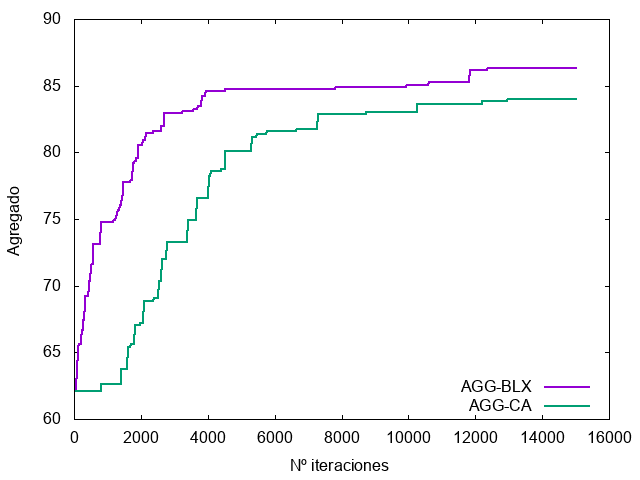
\includegraphics[width=0.7\textwidth]{img/AGG.png}
	\caption{Comparación en una ejecución concreta de los AGG en \textit{ionosphere}}
\end{figure}

En segundo lugar, en los algoritmos genéticos estacionarios se vuelve a producir el efecto comentado anteriormente para los dos tipos de cruce: el cruce aritmético sale perdiendo en todas las ocasiones. Sin embargo, la tasa agregada conseguida por el AGE-CA supera ampliamente a la conseguida por el AGG-CA, mientras que la tasa agregada del AGE-BLX se queda por debajo de la del AGG-BLX en la mayoría de los casos. La mejora observada se puede explicar por la alta presión selectiva que introduce el esquema de reemplazo estacionario, en el que los hijos compiten con el resto de la población para introducirse en ella.\\

\begin{figure}[ht!]
    \centering
    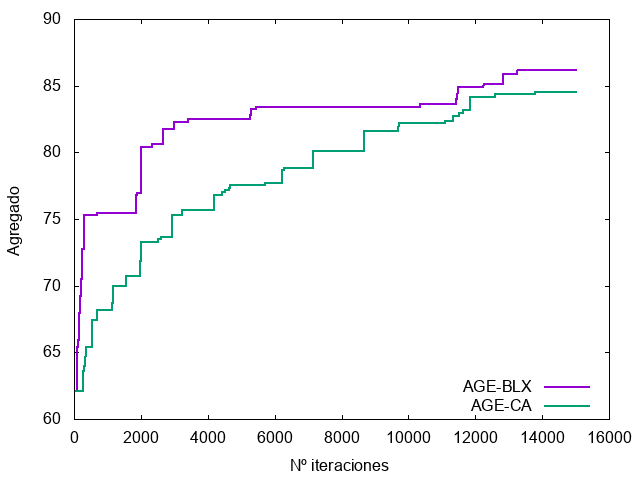
\includegraphics[width=0.7\textwidth]{img/AGE.png}
	\caption{Comparación en una ejecución concreta de los AGE en \textit{ionosphere}}
\end{figure}

En cualquier caso, en la implementación de los algoritmos estacionarios tenemos una probabilidad de mutación relativamente baja (al ser la población intermedia muy reducida), por lo que la diversidad que introducimos en la población es limitada. Esto hace que, tras la convergencia acelerada por el elitismo en el reemplazo, no se consiga mejorar mucho las soluciones y se observen largos periodos de estancamiento, es decir, convergen prematuramente a óptimos locales.\\

En este caso el tiempo de ejecución es similar al de los algoritmos genéticos generacionales, y de nuevo no parece que el tiempo invertido merezca la pena, pues la tasa agregada es menor que la obtenida por la búsqueda local. \\

En tercer lugar, \textbf{los algoritmos meméticos ofrecen una mejora notable de la tasa agregada con respecto al resto de algoritmos considerados} (en esta práctica y en la anterior). Al hibridar un algoritmo genético con alta capacidad de exploración como es el AGG-BLX con un algoritmo que explota mucho las soluciones (búsqueda local) conseguimos una rápida convergencia inicial, con capacidad de mejorar las soluciones y escapar de óptimos locales.\\

Al emplear una búsqueda de baja intensidad y una población reducida conseguimos que el tiempo de ejecución sea incluso inferior al de los algoritmos genéticos.\\

Un detalle que podemos observar es que también hay periodos de estancamiento de las soluciones, motivados probablemente por iteraciones de la búsqueda local que no conducen a mejora, por lo que podríamos pensar en establecer un criterio de parada alternativo que contemple estas situaciones.

\begin{figure}[ht!]
    \centering
    \includegraphics[width=0.7\textwidth]{img/am.png}
	\caption{Comparación en una ejecución concreta de los AM en \textit{ionosphere}}
\end{figure}

En la comparación de los tres algoritmos meméticos no parece haber una tendencia consistente, pues las diferencias entre las tasas agregadas obtenidas es pequeña y puede depender de los procesos aleatorios involucrados.\\

Vemos finalmente una gráfica comparativa de la tasa agregada (sobre el conjunto de entrenamiento) obtenida por todos los algoritmos en función del número de iteraciones realizadas, donde se aprecian las relaciones que hemos comentado anteriormente.\\

\begin{figure}[ht!]
    \centering
    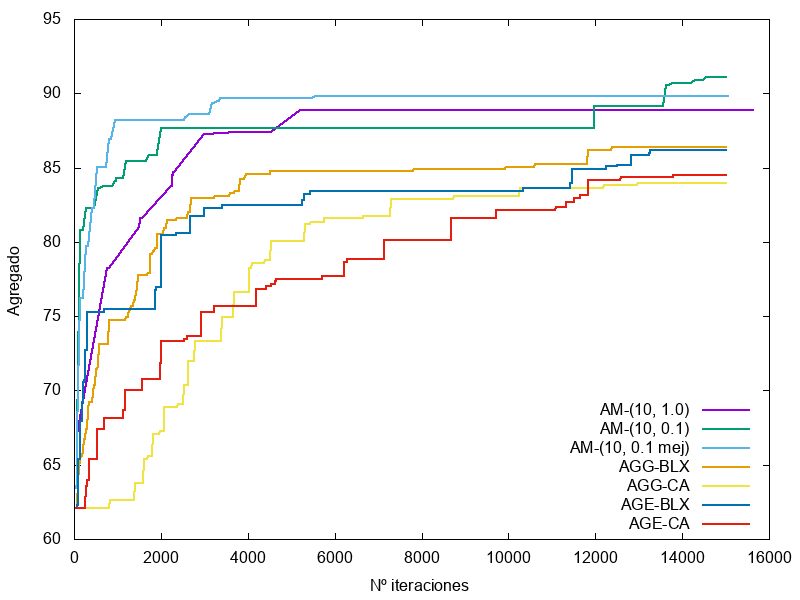
\includegraphics[width=0.7\textwidth]{img/todos.png}
	\caption{Comparación en una ejecución concreta de todos los algoritmos en \textit{ionosphere}}
\end{figure}

Por último, no debemos pensar que el hecho de que los algoritmos genéticos no mejoren mucho los resultados obtenidos por la búsqueda local quiere decir que podamos descartarlos como metaheurísticas adecuadas. Hay muchos factores a tener en cuenta, como son el \textit{sesgo} que puedan tener los conjuntos de datos que utilizamos en favor de un algoritmo u otro, el valor de los distintos parámetros que controlan la ejecución de los algoritmos, la semilla utilizada, etc. 

\end{document}

